\documentclass{VUMIFPSkursinis}
\usepackage{algorithmicx}
\usepackage{algorithm}
\usepackage{algpseudocode}
\usepackage{amsfonts}
\usepackage{amsmath}
\usepackage{bm}
\usepackage{caption}
\usepackage{color}
\usepackage{float}
\usepackage{graphicx}
\usepackage{listings}
\usepackage{subfig}
\usepackage{wrapfig}

% Titulinio aprašas
\university{Vilniaus universitetas}
\faculty{Matematikos ir informatikos fakultetas}
\department{Programų sistemų katedra}
\papertype{Bakalaurinis darbas}
\title{Užsiėmimų lankomumo žymėjimas, panaudojant studentų išmaniuosius telefonus}
\titleineng{Lecture attendance marking using students' smartphones}
\status{4 kurso 2 grupės studentas}
\author{Marijus Siliūnas}
% \secondauthor{Vardonis Pavardonis}   % Pridėti antrą autorių
\supervisor{Dr. Kristina Lapin}
\date{Vilnius – \the\year}

% Nustatymai
% \setmainfont{Palemonas}   % Pakeisti teksto šriftą į Palemonas (turi būti įdiegtas sistemoje)
\bibliography{bibliografija}

\begin{document}
\maketitle

\sectionnonum{Santrauka}

\sectionnonum{Summary}

\tableofcontents

\sectionnonum{Įvadas}

\subsectionnonum{Tyrimo objektas}

Artimojo ryšio technologijų panaudojimas akivaizdinėse studijose.

\subsectionnonum{Temos aktualumas}

Užsiėmimų metu yra žymimas studentų lankomumas. Šį darbą atlieka dėstytojas kiekvieno užsiėmimo metu. Studentai kviečiami vardu ir atsiliepę yra pažymimi kaip dalyvaujantys paskaitoje. Taip nereikalingai užimamas paskaitos laikas bei atsiranda žmogiškos klaidos tikimybė – gali būti pažymėtas ne tas studentas ir pan. Tai ypač svarbu, kuomet galutinis įvertinimas priklauso ir nuo lankomumo. Dėstytojams tai papildoma atsakomybė ir jie turi patys pasirūpinti priemone, kurioje galėtų vesti studentų lankomumo žurnalą. Reikalinga sistema, kurioje būtų suvedami dėstomi dalykai, dėstantys dėstytojai bei studentų grupės ir studentai, vedamas lankomumo žurnalas.

Dar lankomumo žymėjimui kartais yra pasitelkiamas įrankis \textit{Vilniaus universiteto virtuali mokymosi aplinka (VMA)}. Nors jis yra skirtas medžiagos pateikimui bei testų vykdymui pasitaiko, kad sužymėti studentų lankomumui sukuriami tušti testai. Toks sprendimas kaip ir įvykdo keliamą tikslą – sekti studentų lankomumą, tačiau neužtikrina duomenų teisingumo. Studentai gali prisijungti ir užpildyti testą būdami ne užsiėmimo vykimo vietoje.

\subsectionnonum{Darbo tikslas}

Sukurti dalyvaujančių užsiėmime studentų identifikavimo modulį ir juo paremtą studentų lankomumo žymėjimo sistemą, kuri sudarytų pagrindą tolimesnei plėtrai. Išvystyta sistema leis gerinti studentų ir dėstytojų bendradarbiavimą akivaizdinių studijų užsiėmimų metu.

\subsectionnonum{Uždaviniai}

Tikslui pasiekti keliami šie uždaviniai:

\begin{itemize}
	\item Apžvelgti studentų automatizuoto identifikavimo, panaudojant išmaniuosius telefonus, technologines galimybes ir parinkti viena iš jų.
	\item Apžvelgti išmaniųjų telefonų programėlių technologinius įgyvendinimo būdus.
	\item Suformuluoti pagrindinius kuriamo modulio naudojimo scenarijus.
	\item Sukurti studentų identifikavimo modulio vartotojų sąsajos eskizus.
	\item Apibrėžti studentų lankomumo žymėjimo sistemos svarbiausius komponentus bei apžvelgti jų komunikavimo aspektus.
\end{itemize}

\subsectionnonum{Siekiami rezultatai}

\begin{itemize}
	\item Sukurtas automatizuotas studentų lankomumo žymėjimo modelis.
	\item Sukurtos sistemos įgyvendinimo gairės ir sudarytas technologijų rinkinys.
	\item Sukurtas sistemos diegimo vaizdas.
	\item Pateikti studentų identifikavimo modulio vartotojo sąsajos eskizai.
\end{itemize}

\section{Užsiėmime dalyvaujančių studentų identifikavimas}

\subsection{Situacijos analizė}

Šiuo metu studentų užsiėmimų lankomumo sekimas yra dėstytojų atsakomybė. Jie patys turi rasti sprendimą, kaip pažymėti atvykusius į paskaitą studentus. Kaip vieną iš būdų renkasi atspausdintą studentų sąrašą, kuriame pasižymi užsiėmimo vykimo dieną bei atvykusius į užsiėmimą studentus.

Kita lankomumo žymėjimui kartais pasitelkiama priemonė yra \textit{Vilniaus universiteto virtuali mokymosi aplinka (VMA)}. Nors ji yra skirtas medžiagos pateikimui bei testų vykdymui, pasitaiko, kad sužymėti studentų lankomumui sukuriami tušti testai – prašoma įvesti tik lietuvos studento pažymėjimo numerį arba vardą ir pavardę. Toks sprendimas kaip ir įvykdo keliamą tikslą – sekti studentų lankomumą, tačiau neužtikrina duomenų teisingumo. Studentai gali prisijungti ir užpildyti testą būdami ne užsiėmimo vykimo vietoje.

// TODO: Esamos situacijos palyginimas, kas vyksta (Esami scenarijai), problemas numeruoti, neišnaudotos galimybės numeruotos ir paskui parašom, ką pataisėm, iš ko padarėm tokias išvadas

Lankomumo žymėjimas yra pasikartojantis ir toks pat procesas, kurį galima visiškai automatizuoti. Norint automatizuoti lankomumo žymėjimo procesą, pirmiausia reikia pasirinkti priemonę, kurią galime unikaliai identifikuoti ir susieti su studento vardu ir pavarde, esančias dėstytojo sąraše. Lengviausiai prieinamos studentams priemonės yra:

\begin{itemize}
	\item Lietuvos studento pažymėjimas
	\item Išmanusis telefonas
\end{itemize}

Automatizavus lankomumo žymėjimo procesą, pasitelkiant vieną iš pateiktų priemonių, būtų supaprastinamas dėstytojų darbas bei taupomas užsiėmimo laikas. 

\subsection{Lietuvos studento pažymėjimas}
Vienas iš būdų yra Lietuvos studento pažymėjimo (toliau - LSP) panaudojimas studento identifikavimui. Naujo pavyzdžio LSP turi integruotą NFC (angl. \textit{Near Field Communication}) technologiją.  Jos pagalba galime nuskaityti LSP unikalų identifikavimo numerį ir pagal jį identifikuoti studentą. Identifikavus studentą sistemoje pažymimas jo dalyvavimas paskaitoje.

Visi studentai pradėję studijuoti įsigyja LSP todėl studentams toks procesas nesukeltų jokių nepatogumų. Pagrindinis trūkumas, kad universiteto auditorijose turėtų būti įdiegti \textit{NFC} skaitytuvai arba dėstytojai turi turėti išmaniuosius telefonus su įdiegta \textit{NFC} technologija. Norint efektyviai atlikti žymėjimą turėtų būti įrengtas ne vienas, nes pažymėti galima tik po vieną studentą. Taip pat studentai gali pamiršti pasiimti su savimi LSP.

\subsection{Išmanusis telefonas}
Kitas būdas galėtų būti panaudojant Bluetooth technologiją. Pati technologija nėra nauja, tačiau vis tobulinama. Beveik visi šiuo metu naudojami mobilieji telefonai turi integruotą šią technologiją. Mobiliuosius telefonus turi visi studentai. Kiekvienas įrenginys, kuriame yra integruota Bluetooth technologija, turi savo unikalų identifikavimo numerį, kurį galima nuskaityti. Kaip ir prieš tai pateiktu būdu - šį numerį reikėtų susieti su studento vardu ir pavarde.

Universiteto auditorijose taip pat turėtų būti įdiegiami skaitytuvai, kurie nuskaitytų studentų mobiliųjų telefonų unikalius identifikacinius numerius. Tokio skaitytuvo tereikėtų vieno auditorijoje, nes mobiliųjų telefonų siunčiamus signalus Bluetooth ryšius galima nuskaityti visus vienu metu. Nors studentai turėtų įjungti šią technologiją telefone, pats procesas vyktų žymiai efektyviau ir paprasčiau.

\subsection{LSP ar išmanusis telefonas?}
Pateikti būdai turi ir privalumų, ir trūkumų. Visgi tinkamesnis būdas identifikuoti studentus yra pasitelkus Bluetooth technologiją, nes:

\begin{itemize}
	\item Auditorijose nereikia įrengti specialios įrangos
	\item Greitesnis identifikavimas, nesusidaro eilės prie skaitytuvų
\end{itemize}

Verta paminėti, kad šie būdai nėra priešinami, o laikomi alternatyvomis. Jei telefonas išsikrovęs, galima būtų identifikuoti su LSP. Tokiu atveju turėtų būti įrengti \textit{NFC} technologijos skaitytuvai.

\subsection{Sistemos naudojimo vizija}

\begin{figure}[H]
	\centering
	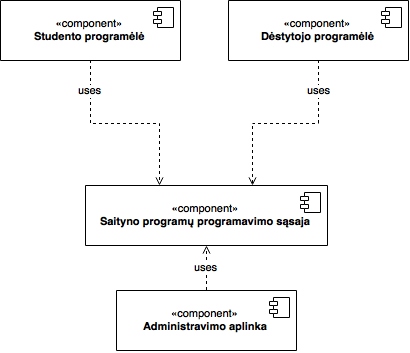
\includegraphics[scale=0.5]{img/kursinio_component}
	\caption{Sistemos komponentai}
	\label{img:componentDiagram}
\end{figure}

Pagal pateiktą \textit{UML} sistemos komponentų diagramą (\ref{img:componentDiagram} pav.) matome, kad sistemą sudaro keturi pagrindiniai komponentai – studento ir dėstytojo telefonai, saityno programų programavimo sąsają ir administravimo aplinka.

\subsection{Mobilioji programėlė studentams} \label{StudentApp}
Toks proceso įgyvendinimas prasideda nuo programėlės sukūrimo išmaniesiems telefonams. Taip pat svarbu, kad programėlė ne tik padėtų identifikuoti studentą, tačiau būtų kuo paprastesnė (reikėtų atlikti kuo mažiau veiksmų) naudotojui.

Kiekvienas įrenginys turintis integruotą Bluetooth technologiją turi ir unikalų MAC (angl. \textit{Media Access Control}) adresą, dar vadinamą fiziniu adresu. Kadangi šis adresas kievienam įrenginiui yra unikalus, tai juo galime naudotis norint identifikuoti studentus. Norint susieti studento mobilųjį telefoną su jo paskyra sistemoje studentas įsidiegia programėlę. Programėlėje studentas prisijungia prie savo paskyros ir susieja mobilųjį telefoną. Programėlė nuskaito telefono Bluetooth MAC adresą ir kartu su studento identifikavimo numeriu (gaunamas prisijungus prie paskyros) siunčia į sistemą. Sistema gautą MAC adresą priskiria tam studentui. Programėlės pagrindinė funkcija yra susieti telefoną su paskyra. Tuo pačiu galima pateikti studento tvarkaraštį, lankomumo ataskaitą.

Norint, kad sistema galėtų naudotis kuo daugiau studentų, programėlė turi būti palaikoma skirtingose įrenginiuose bei operacinėse sistemose. Pačios populiariausios išmaniųjų įrenginių operacinės sistemos yra \textit{Android} ir \textit{iOS}. Taip pat gana plačiai naudojama \textit{Windows Phone} operacinė sistema \cite{MarketShareByOS}.

\subsubsection{Programėlių kūrimas pagal operacinę sistemą}

\subsubsubsection{Android}
Tai yra populiariausia, apie 80 procentų rinkos užimanti \cite{MarketShareByOS}, operacinė sistema. Ši platforma yra atviro kodo ir prižiūrima \textit{Google} kompanijos. \textit{Android} operacinė sistema diegiama į tokių kaip \textit{LG}, \textit{Sony} ir kitų gamintojų išmaniuosius telefonus. Šiai platformai programėlės kuriamos \textit{Java} programavimo kalba. Programavimo aplinkai kūrėjai siūlo nemokamą įrankį \textit{Android Studio} bei pamokų ciklą pirmąjai programėlei sukurti.

\subsubsubsection{iOS}
Antra pagal populiarumą, apie 15 procentus rinkos turinti \cite{MarketShareByOS}, operacinė sistema. Ši platforma yra palaikoma ir sukurta \textit{Apple} korporacijos. Programėlės kuriamos \textit{Objective-C} arba \textit{Swift} programavimo kalbomis.

\subsubsubsection{Windows Phone}

Trečia pagal populiarumą, apie 3 procentus išmaniųjų įrenginių rinkos užimanti \cite{MarketShareByOS}, operacinė sistema. Tai yra \textit{Microsoft} korporacijos produktas. Operacinė sistema diegiama \textit{Nokia} korporacijos \textit{Lumia} išmaniųjų telefonų linijoje. Programavimo kalba – \textit{C\#}.

\subsubsection{Viena programėlė – visoms operacinėms sistemoms}
Studentai turi daug ir skirtingų išmaniųjų telefonų, todėl sistema turi palaikyti kuo daugiau įrenginių. Mūsų atveju taip pat reikalinga, kad naudojimąsis sistema būtų kuo prieinamesnis. Neseniai pradėtos kurti technologijos leisiančios rašyti kodą vienai programėlei ir ji veiktų populiariausiose \cite{MarketShareByOS} išmaniųjų įrenginių operacinėse sistemose. Kol kas nėra tiek išvystyta technologija, tačiau šiuo metu galime su nedidelėmis korekcijomis sukurti programėlę tinkamą populiariausioms išmaniųjų irenginių operacinėms sistemoms.

\subsubsubsection{Savoji programėlė}

Sparčiai tobulėjanti platforma, skirta kurti programėles \textit{Android}, \textit{iOS} ir \textit{Windows Phone} operacinėms sistemoms, tai \textit{Xamarin} \cite{xamarin}. Naudojantis šia platforma galima kurti visoms trims mobiliosioms operacinėms sistemoms savąsias (angl. \textit{native}) programėles. Šiuo atveju programėlės yra rašomos \textit{C\#} programavimo kalba, o programinė įranga, reikalinga kurti programėles, yra nemokama. Vidutiniškai 75 procentai programėlės kodo yra naudojama bendrai tarp operacinių sistemų. Platforma suteikia pilną priėjimą prie įrenginio operacinės sistemos programų programavimo sąsajos (angl. \textit{Application Programming Interface, API}). Vartotojo sąsają galima kurti pagal operacinės sistemos standartus arba naudojant platformos kūrėjų įrankį \textit{Xamarin.Forms}.

\subsubsubsection{Saityno programėlė} \label{webApp}

Priklausomai nuo poreikių, galima sukurti tinklalapį pritaikytą mobiliesiems įrenginiams. Kuriant galima pasitelkti karkasus, skirtus kurti būtent tokias saityno programėles, pavyzdžiui: \textit{Bootstrap}, \textit{Foundation} \cite{cssFrameworks}. Tai yra greitas ir pigus būdas, prieinamas iš visų operacinių sistemų. Tačiau tinkamas tik tuomet, kai nereikia arba reikalingos elementarios (garsas, failai įrenginio atmintyje) sąsajos su įrenginiu. Taip pat programėlė laikoma serveryje ir yra parsiunčiama į telefoną kiekvienos užklausos metu, todėl gali sukelti nepatogumų, nes naudojant mobilųjį internetą dažniausiai duomenų kiekis yra ribojamas.

\subsubsubsection{Hibridinė programėlė}

Hibridinė programėlė – tai saityno programėlė, tačiau integruota į 	savą programėlę. Tai suteikia galimybę priėjimą prie įrenginio operacinės sistemos programų programavimo sąsajos. Tokiu būdu mes galime pasiekti išmaniojo įrenginio resursus.

Vienas iš labiausiai paplitusių karkasų yra \textit{Ionic} \cite{hybridFrameworks}. Naudojantis šiuo karkasu galime programėlę kurti kaip tinklalapį, programuojant \textit{JavaScript} programavimo kalba bei rašant \textit{HTML} ir \textit{CSS} kodą vartotojo sąsajai kurti.

\subsubsubsection{Tinkamiausio būdo parinkimas}

Mūsų kuriamos sistemos atveju svarbiausia gera programėlės integracija su įrenginio komponentais, o konkrečiau – įrenginio \textit{Bluetooth} ryšio moduliu. Taip pat labai svarbu, kad programėlė būtų kuo prieinamesnė – turi būti palaikomos populiariausios išmaniųjų telefonų operacinės sistemos.

\begin{table}[H]
	\centering
	\begin{tabular}{ | r | c | c | c | }
		\hline
		& Savoji & Saityno & Hibridinė \\
		\hline
		\textbf{Prieinamas \textit{Bluetooth} ryšys} & + &  & + \\
		\hline
		Veikia visose populiariausiose operacinėse sistemose & + & + & + \\
		\hline
		Kūrimo įrankiai yra nemokami & + & + & + \\
		\hline
	\end{tabular}
	\caption{Programėlių kūrimo būdų palyginimas}
	\label{appCompare}
\end{table}

Norint identifikuoti studentus panaudojant jų išmaniuosius telefonus programėlei būtinas priėjimas prie įrenginio \textit{Bluetooth} ryšio modulio, todėl saityno programėlė mums netinka. Hibridines programėles galima kurti greičiau ir paprasčiau nei savąsias, tačiau jų veikimo sparta bei vientisumas gali kelti nepatogumų naudotojams. Taip pat yra sudėtingiau išnaudoti įrenginio ir jo operacinės sistemos teikiamas funkcijas, pasiekiamas per aplikacijų programavimo sąsaja. Todėl tinkamiausias būdas kurti programėlę sistemai yra naudojant \textit{Xamarin} platformą. Ji leis sukurti intuityvesnę, vientisesnę bei patikimesnę programėlę.

\subsubsection{Savosios programėlės detalieji naudojimo scenarijai}

\subsubsubsection{Prisijungimas}

Įdiegus ir pirmą kartą programėlę paleidus naudotojui atidaromas prisijungimo langas (\ref{img:loginView} pav.). Studentas suveda prisijungimo vardą bei slaptažodį. Spaudžia prisijungti. Sistemai grąžinus sėkmingą pranešimą, programėlėje išsaugomi prisijungimo duomenis. Kitą kartą paleidus programėlę prisijungimas vyksta automatiškai.

\subsubsubsection{Įrenginio susiejimas}

Pagrindiniame programėlės lange (\ref{img:mainView} pav.) matome pranešimą, kad nėra susietas įrenginys su paskyra. Spaudžiame „Susieti įrenginį“. Programėlė surenka reikalingą informaciją apie įrenginį (\textit{Bluetooth MAC} adresą) ir siunčia užklausą į sistemos aplikacijų programavimo sąsają. Grąžinama žinutė apie sėkmingą arba nesėkmingą įrenginio susiejimą su paskyra.

\textbf{Alternatyvus scenarijus:} Prisijungus programėlėje, atidarome meniu (\ref{img:menuView} pav.) paspausdami ant meniu piktogramos viršutinėje juostoje. Atsidariusiame meniu pasirenkame „Susieti įrenginį“.

\subsubsubsection{Lankomumo pažymėjimas}

\textbf{Rankinis scenarijus:} Studentas atėjęs į paskaitą įsijungia programėlę bei įrenginio Bluetooth ryšį. Pagrindiniame lange (\ref{img:mainView} pav.) spaudžia mygtuką „Dalyvauju“. Programėlė ieško skaitytuvo ir nuskaito jo siunčiamą informaciją: paskaitos pavadinimą, dėstytojo vardą ir pavardę. Rodomas patvirtinimo langas su šia informacija. Studentas spaudžia „Taip“. Patvirtinimas siunčiamas į sistemą ir pažymimas studento dalyvavimas paskaitoje.

\textbf{Automatizuotas scenarijus:} Jei studentas išmaniajame telefone įjungęs \textit{Bluetooth} ryšį ir yra susiejęs įrenginį su paskyra, skaitytuvas aptikęs įrenginį automatiškai pažymi studento dalyvavimą užsiėmime.

\subsubsubsection{Paskyros peržiūra}

Programėlėje studentas taip pat gali peržiūrėti savo paskyrą meniu (\ref{img:menuView} pav.) spausdamas mygtuką „Paskyra“.

\subsubsection{Savosios programėlės vartotojo sąsaja}

Studentams skirtos programėlės pagrindinės funkcijos – pasižymėti dalyvavimą užsiėmime bei susieti įrenginį su studento vardu ir pavarde. Projektuojant vartotojo sąsają pagrindinis dėmesys skiriamas šių veiksmų paprastumui, stengiamasi, kad užduočių atlikimui reikėtų kuo mažiau veiksmų. Vartotojo sąsają, naudojant \textit{Xamarin} platformą, galima kurti dviem būdais:

\begin{itemize}
	\item Kiekvienos operacinės sistemos vartotojo sąsajos kūrimo įrankiu
	\item \textit{Xamarin} platformos kūrėjų kurtu įrankiu \textit{Xamarin Forms}
\end{itemize}

Kuriant vartotojo sąsają kiekvienos operacinės sistemos vartotojo sąsajos kūrimo įrankiu kyla nepatogumas, kad reikia tuos pačius langus aprašyti tris kartus. Vartotojo sąsaja kuriant \textit{Xamarin Forms} įrankiu, visuose įrenginiuose, nepriklausomai nuo operacinės sistemos, vartotojo sąsaja bus atvaizduojama ta pati ir aprašoma vieną kartą. Šio įrankio naudojimas pagreitina įgyvendinimą, nes nebereikia atskirai kurti kiekvienai operacinei sistemai vartotojo sąsajos atskirai. Tuo pačiu reikia atsižvelgti į tai, jog dėl tos pačios priežasties įrenginių ekrano dydžiai labai skirtingi.

\begin{figure}[H]
	\centering
	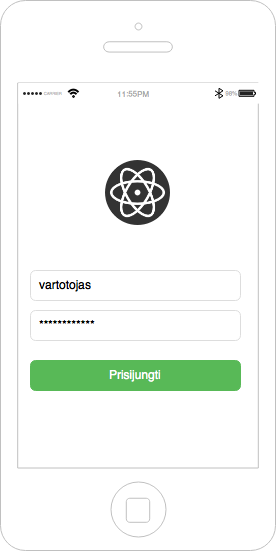
\includegraphics[scale=0.5]{img/kursinio_app_login}
	\caption{Prisijungimo langas}
	\label{img:loginView}
\end{figure}

Prisijungimo langas (\ref{img:loginView} pav.) matomas tik pirmą kartą prisijungiant arba po atsijungimo. Naudotojui reikia suvesti prisijungimo vardą bei slaptažodį ir paspausti mygtuką „Prisijungti“. Jei pateikti duomenys teisingi, atidaromas pagrindinis langas (\ref{img:mainView} pav.). Kitu atveju rodomas klaidos pranešimas.

\begin{figure}[H]
	\centering
	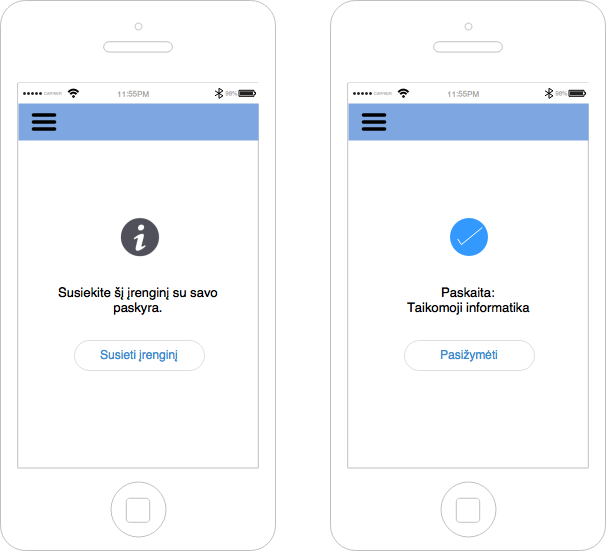
\includegraphics[scale=0.5]{img/kursinio_app_main}
	\caption{Pagrindinis langas}
	\label{img:mainView}
\end{figure}

Pagrindiniame lange (\ref{img:mainView} pav.), priklausomai nuo to, ar esame susieję įrenginį su mūsų paskyra, matome arba pranešimą, kad turime susieti įrenginį su paskyra arba paskaita, kurioje galime pasižymėti, kad dalyvaujame.

\begin{figure}[H]
	\centering
	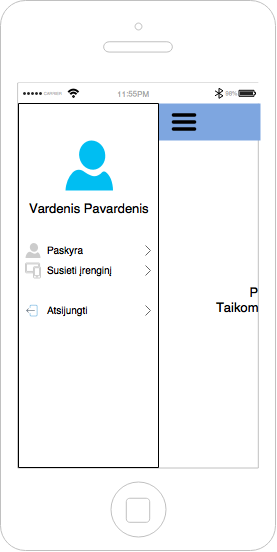
\includegraphics[scale=0.5]{img/kursinio_app_menu}
	\caption{Meniu}
	\label{img:menuView}
\end{figure}

Meniu (\ref{img:menuView} pav.) pateikiamas prisijungusio naudotojo vardas ir pavardė bei nedidelė profilio nuotrauka. Meniu atidaryti galima viršutinėje juostoje paspaudus meniu ikoną.

\subsection{Skaitytuvas – išmanusis telefonas} \label{TeacherApp}
Kitas svarbus komponentas, norint identifikuoti studentus, naudojant \textit{Bluetooth} ryšį – skaitytuvas. Tai galėtų būti atskiras prietaisas arba tiesiog išmanusis telefonas. Reikalinga sukurti atskirą programėlę, kuri būtų įdiegta dėstytojo išmaniajame telefone.

Paskaitos metu programėlė nuskaito įrenginius esančius patalpoje ir siunčia įrenginių sąrašą su jų \textit{Bluetooth MAC} adresais į sistemą, kur gautas unikalus identifikatorius susiejamas su studento paskyra ir pažymimas jo dalyvavimas paskaitoje. Norint tai įgyvendint, dėstytojas taip pat turi turėti savo paskyrą sistemoje. Paskyroje pridedamos paskaitos, priskiriamos grupės bei studentai.

Kaip ir programėlė skirta studentams, taip ir skirta dėstytojams turi būti kuo prieinamesnė. Todėl jos kūrimui taip pat pasirinkta \textit{Xamarin} platforma.

\subsubsection{Skaitytuvo programėlės funkcijos}

\subsubsubsection{Prisijungimas}

Įdiegus ir pirmą kartą programėlę paleidus naudotojui atidaromas prisijungimo langas (\ref{img:scannerLoginView} pav.). Dėstytojas suveda prisijungimo vardą bei slaptažodį. Spaudžia prisijungti. Sistemai grąžinus sėkmingą pranešimą, programėlė išsisaugo prisijungimo duomenis arba prieigos raktą (priklausomai nuo sistemos vidinės pusės įgyvendinimo). Kitą kartą paleidus programėlę prisijungimas vyksta automatiškai.

\subsubsubsection{Paskaitos pradžia}

Paleidus programėlę ir prisijungus (automatiškai arba suvedus prisijungimo duomenis) pagrindiniame lange (\ref{img:scannerMainView} pav.) naudotojas paspaudžia ant mygtuko „Paskaita“, atidaromas paskaitos pasirinkimo langas (\ref{img:scannerMainView} pav.), išsirenka paskaitą ir ant jos paspaudžia. Atidaromas pagrindinis langas (\ref{img:scannerMainView} pav.) ir rodoma pasirinkta paskaita. Taip pat pasirenkama grupė. Parinkus paskaitą ir grupę naudotojas spaudžia „Pradėti paskaitą“. Programėlė pradeda skleisti informaciją \textit{Bluetooth} ryšiu. Rodomas paskaitos langas su pasižymėjusiais studentais.

\textbf{Alternatyvus scenarijus:} Pradėjus paskaitą periodiškai ieškoma įrenginių su įjungtu \textit{Bluetooth} ryšiu. Rastų įrenginių \textit{Bluetooth MAC} adresai siunčiami į sistemą.

\subsubsubsection{Paskaitos pabaiga}

Paskaitos lange (\ref{img:scannerLectureView} pav.) naudotojas spaudžia „Užbaigti paskaitą“. Rodomas patvirtinimo pranešimas, spaudžia „Užbaigti“. Programėlė nusiunčia užklausą į sistemą dėl paskaitos užbaigimo. Rodomas pranešimas su sėkmingo arba nesėkmingo užbaigimo tekstu. Atidaromas pagrindinis langas (\ref{img:scannerMainView} pav.).

\subsubsection{Skaitytuvo programėlės vartotojo sąsaja}

Projektuojant skaitytuvo programėlės vartotojo sąsają stengtąsi pateikti taip, kad reikėtų kuo mažiau veiksmų norint atlikti pagrindines užduotis. Svarbiausios programėlės funkcijos yra paskaitos pasirinkimas bei studentų įrenginių aptikimas, todėl šioms užduotims skirtas pagrindinis dėmesys.

Programėlėje išlaikomas ta pati struktūra, kaip ir studentų programėlėje. Kad nebūtų painiojamos tarpusavyje, naudojamos kitos spalvos.

\begin{figure}[H]
	\centering
	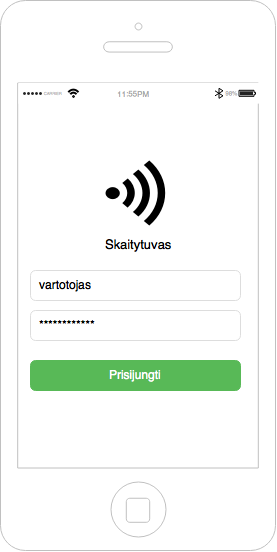
\includegraphics[scale=0.5]{img/kursinio_app_dest_login}
	\caption{Prisijungimo langas}
	\label{img:scannerLoginView}
\end{figure}

Prisijungimo langas (\ref{img:scannerLoginView} pav.) toks pat kaip ir studentų programėlėje.

\begin{figure}[H]
	\centering
	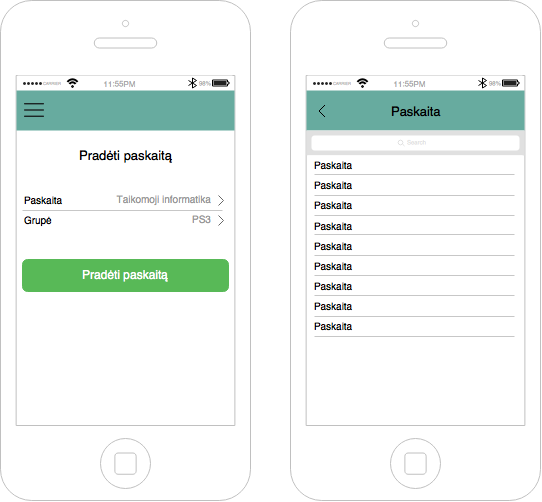
\includegraphics[scale=0.5]{img/kursinio_app_dest_main}
	\caption{Pagrindinis langas (kairėje) ir paskaitos pasirinkimo langas (dešinėje)}
	\label{img:scannerMainView}
\end{figure}

Pagrindiniame lange (\ref{img:scannerMainView} pav.) galime pasirinkti paskaitą ir grupę. Grupės pasirinkimo langas yra analogiškas paskaitos pasirinkimo langui (\ref{img:scannerMainView} pav.) – taip pat pateikiama paieška ir dėstytojų grupių sąrašas. Verta pažymėti, kad grupės pasirinkimo lange pateikiamas sąrašas grupių, kurios yra priskirtos pasirinktai paskaitai.

\begin{figure}[H]
	\centering
	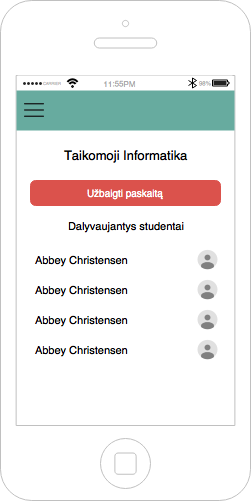
\includegraphics[scale=0.5]{img/kursinio_app_dest_lecture}
	\caption{Paskaitos langas}
	\label{img:scannerLectureView}
\end{figure}

Iš pagrindinio lango (\ref{img:scannerMainView} pav.) patenkama į paskaitos langą (\ref{img:scannerLectureView} pav.). Šiame lange matome paskaitos pavadinimą, paskaitos užbaigimo mygtuką bei dalyvaujančių (pažymėtų) studentų sąrašą.

\section{Sistemos vidinė pusė}

// TODO: Diegimo instrukcija serverio

Apžvelgėme, kokiu būdu ir kokiomis priemonėmis sistemos naudotojai galės naudotis sistema. Bet visa tai neveiks be pagrindinės sistemos dalies, atsakingos už duomenų saugojimą, apdorojimą ir pateikimą.

\begin{figure}[H]
	\centering
	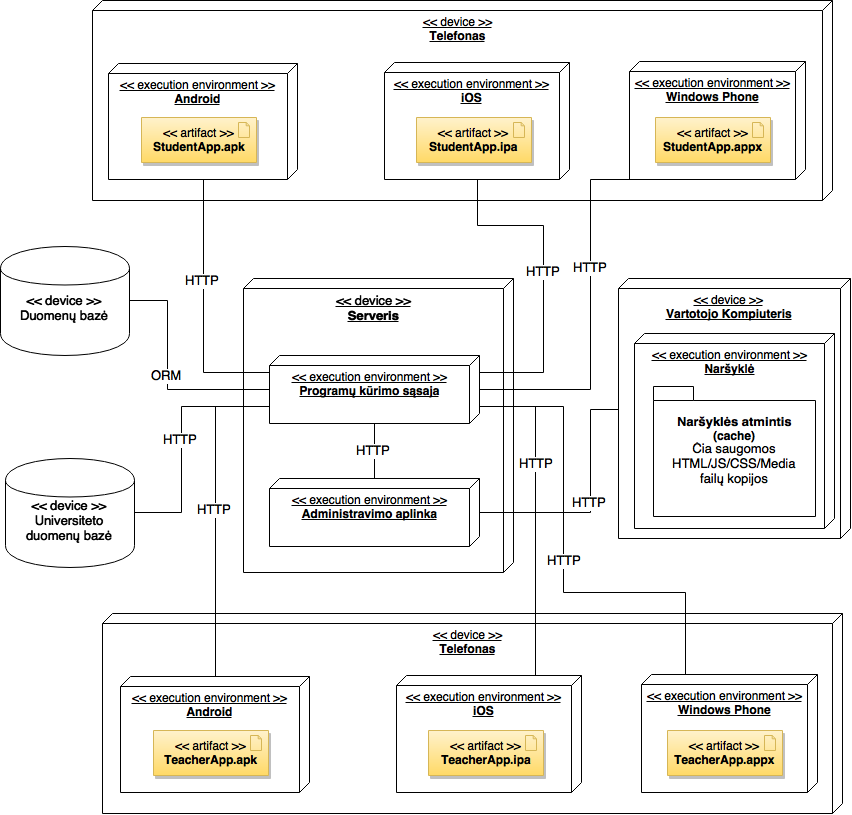
\includegraphics[scale=0.5]{img/kursinio_deployment.png}
	\caption{Sistemos diegimo vaizdas}
	\label{img:deployment}
\end{figure}

Pagal pateiktą diegimo diagramą (\ref{img:deployment} pav.) matome, kad visą sistemą sudaro trys pagrindiniai moduliai: mobiliosios programėlės (aprašytos \ref{StudentApp} ir \ref{TeacherApp} poskyriuose), programų kūrimo sąsaja bei administravimo aplinka.

\subsection{Sistemos esybės}

\begin{figure}[H]
	\centering
	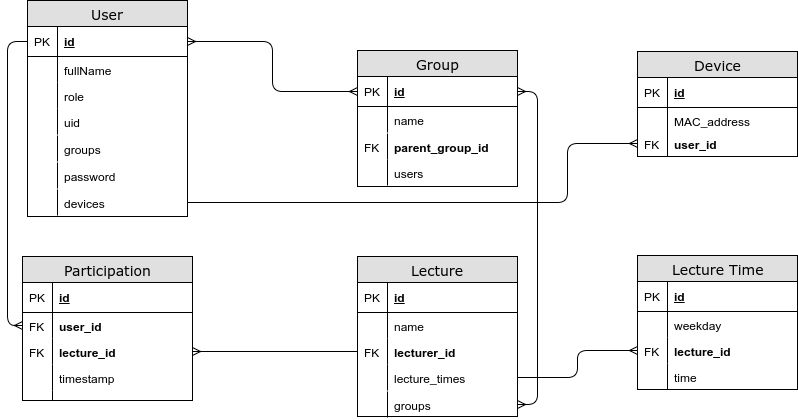
\includegraphics[scale=0.5]{img/Bakalauro-ER.png}
	\caption{Sistemos esybių ryšiai}
	\label{img:er-diagram}
\end{figure}

Kaip matome pateiktoje esybių ryšių diagramoje (\ref{img:er-diagram} pav.) sistemos numatytoms funkcijos įgyvendinti reikalingos išvardintos esybės su nurodytais laukais:

\begin{itemize}
    \item Naudotojas
    \begin{itemize}
        \item Identifikatorius
        \item Pilnas vardas
        \item Rolė (studentas, dėstytojas)
        \item Unikalus identifikatorius
        \item Grupių, kurioms priklauso, sąrašas
        \item Slaptažodis
        \item Įrenginiai
    \end{itemize}
    \item Grupė
    \begin{itemize}
        \item Identifikatorius
        \item Pavadinimas
        \item Tėvinė grupė
        \item Naudotojai
    \end{itemize}
    \item Įrenginys
    \begin{itemize}
        \item Identifikatorius
        \item \textit{MAC} adresas
        \item Naudotojas
    \end{itemize}
    \item Paskaita
    \begin{itemize}
        \item Identifikatorius
        \item Pavadinimas
        \item Dėstytojas
        \item Paskaitos laikas
        \item Grupių sąrašas
    \end{itemize}
    \item Paskaitos laikas
    \begin{itemize}
        \item Identifikatorius
        \item Paskaita
        \item Savaitės diena
        \item Paskaitos laikas
    \end{itemize}
    \item Dalyvavimo įrašas
    \begin{itemize}
        \item Identifikatorius
        \item Naudotojas
        \item Paskaita
        \item Įrašo laikas
    \end{itemize}
\end{itemize}

Naudotojas turi roles – \textit{studento} arba \textit{dėstytojo}. Jei naudotojo rolė \textit{studentas}, tai lietuvos studento pažymėjimo numeris įvedamas kaip unikalus identifikatorius, kitu atveju – įvedamas dėstytojo darbuotojo numeris.

Grupės gali turėti tėvines grupes, todėl tai gali atstoti universiteto kursus ir kurso grupes. Paskaita gali būti sukurta visam kursui ar net keliems kursams arba kurso grupei ar kelioms grupėms.

Paskaitai priskiriamos grupės, dėstytojas. Taip pat sukuriami ir priskiriami paskaitos laikai – nurodoma savaitės diena bei dienos laikas. Ši informacija padės automatizuoti paskaitų lankomumo sekimo aktyvavimo automatizavimą.

Dalyvavimo įrašas sukuriamas, kuomet dėstytojo programėlė arba skaitytuvas aptinka studento telefoną ir atsiunčią užklausą serveriui. Priskiriamas naudotojas (su \textit{studentas} role), paskaita bei pažymima, kokiu laiku studentas atvyko į paskaitą.

\subsection{Saityno programų programavimo sąsaja} \label{webApi}

Visas bendravimas tarp programėlių ir pagrindinio sistemos modulio vyksta per programų programavimo sąsają. Šis sistemos modulis turi būti sukurtas taip, kad būtų galima nesunkiai įtraukti naują modulį į sistemos architektūrą. Taip pat svarbūs kriterijai renkantis sprendimą:

\begin{itemize}
	\item Maža duomenų apsikeitimo apimtis – turi būti taupomi tinklo ištekliai
	\item Užklausų apdorojimo ir atsakymo siuntimo sparta
\end{itemize}

Saityno programų programavimo sąsaja (angl. \textit{Web Application Programming Interface}) yra dažnas sprendimas tokioms sistemoms įgyvendinti. Tai yra sąsaja, susidedanti iš vieno ar daugiau viešai pasiekiamų prieigos taškų (angl. \textit{endpoint}), su apibrėžta užklausos – atsakymo žinučių sistema. Yra du pagrindiniai saityno programų programavimo sąsajų tipai: \textit{SOAP (Simple Object Access Protocol)} saityno paslaugos ir \textit{REST (Representational State Transfer)} saityno ištekliai.

\subsubsection{Saityno programų programavimo sąsajų tipai}

\subsubsubsection{SOAP}

Tai supaprastintas protokolas skirtas apsikeisti struktūrizuota informacija decentralizuotoje aplinkoje. Šis protokolas naudoja \textit{XML (EXtended Markup Language)} technologiją apibrėžti žinučių karkasą leidžiantį kurti žinutes, kuriomis galima apsikeisti su daugybe kitų protokolų. \textit{SOAP} projektuotas taip, kad būtų nepriklausomas nuo jokios programavimo kalbos ar modelio \cite{SoapDocs}.

Kaip rašoma straipsnyje \cite{SoapRest} – nors modelis kurtas, kad bendravimas tarp sistemų būtų paprastesnis, tačiau naudojant \textit{XML} technologiją užklausų siuntimas gali tapti labai sudėtingas. Priklausomai nuo programavimo kalbos, gali tekti visą užklausą sukurti rankiniu būdu. Kita vertus, protokolas yra sukurtas \textit{Microsoft} korporacijos, todėl implementuojant \textit{SOAP C\#} programavimo kalboje, \textit{XML} kodo beveik netenka matyti.

Viena svarbiausių \textit{SOAP} funkcijų ir privalumų – įtaisytas klaidų apdorojimas. Jei siunčiamoje užklausoje yra klaida, gautame atsakyme pateikiama informacija, kuri gali padėti greitai rasti ir ištaisyti klaidą.

\subsubsubsection{REST}

\textit{REST} metodas leidžia dar paprasčiau apsikeisti žinutėmis tarp programų. Dažnai užtenka pagal taisykles sudaryto universalaus adreso. Kuomet reikia pateikti daugiau informacijos dažnai naudojamas \textit{JSON (JavaScript Object Notation)} formatas. Šis būdas yra patogus tuo, kad galima siųsti ir gauti žinutes forma, kurią lengva sintaksiškai analizuoti programavimo kalboje su kuria yra kuriama programa \cite{SoapRest}.

Naudojant \textit{REST} saityno išteklius yra lengviau įsisavinti metodą nei \textit{SOAP} atveju, taip pat yra efektyvesnis veikimas (galima siųsti mažesnes žinutes) bei ištekliai yra prieinamesni, nereikalingos papildomos programinės priemonės naudojimui. Dėl šių priežasčių tai yra tinkamesnis variantas sistemos saityno programų programavimo sąsajai sukurti.

\subsubsection{Programų programavimo sąsajos valdikliai}

\begin{figure}[H]
	\centering
	\includegraphics[scale=0.6]{img/api-class.png}
	\caption{Programų programavimo sąsajos valdikliai}
	\label{img:api-class-diagram}
\end{figure}

Kuriant programų programavimo sąsają vadovaujantis \textit{REST} metodu nesunku numatyti reikalingus valdiklius kartu su prieigos taškais. Kiekviena esybė arba jų rinkinys turi savo atskirą valdiklį. Pagal pateiktą klasių diagramą (\ref{img:api-class-diagram} pav.) matome, kad sistemos funkcionalumui įgyvendinti reikalingi keturi valdikliai:

\begin{itemize}
    \item Naudotojo valdiklis
    \item Grupės valdiklis
    \item Paskaitos valdiklis
    \item Dalyvavimo įrašo valdiklis
\end{itemize}

\subsubsubsection{Naudotojo valdiklis}

Naudotojo valdiklis skirtas naudotojų sukūrimui, ištrynimui, redagavimui bei skaitymui. Taip pat šis valdiklis atsakingas už naudotojo įrenginių valdymą. Naudotojai su role \textit{studentas} gali tik skaityti duomenis (ne visus) apie kitus naudotojus ir valdyti savo įrenginius.

Dar viena svarbi šio valdiklio atsakomybė – duomenų įkėlimas. \textit{Dėstytojai} gali įkelti duomenis apie studentus ir taip iškart sukurti \textit{studentų} paketą. Duomenys gali būti įkeliami iš failo. Apie tai plačiau \ref{data-import} skyriuje.

\subsubsubsection{Grupės valdiklis}

Grupės valdiklis leidžia naudotojams, kurių rolė yra \textit{dėstytojas}, kurti naujas grupes, jas redaguoti ir trinti. Skaityti grupės informaciją gali ir naudotojai su role \textit{studentas}, tačiau šie naudotojai gali matyti tik tų grupių, kurioms priklauso, duomenis. \textit{Dėstytojai} gali sukurti pogrupius (priskirti grupei tėvinę grupę) ir pridėti arba išimti naudotojus iš grupės.

\subsubsubsection{Paskaitos valdiklis}

Šis valdiklis naudotojams su role \textit{dėstytojas} leidžia sukurti naujas paskaitas, jas modifikuoti ir ištrinti. Šis valdiklis dar atsakingas už paskaitos laikų kūrimą – kuriant paskaitą sukuriami ir nurodyti paskaitos vykimo laikai. \textit{Dėstytojai} taip pat gali valdyti užsiėmimui priskirtas grupes. \textit{Studentai} gali tik skaityti informaciją apie paskaitą – koks dėstytojas veda užsiėmimą bei kokiu laiku vyks užsiėmimas.

\subsubsubsection{Dalyvavimo įrašo valdiklis}

Dalyvavimo įrašo valdiklis \textit{studentams} leidžia tik gauti duomenis apie įrašus, kurie yra susiję su jais. Kurti naujus įrašus gali tik naudotojai su \textit{dėstytojo} role. Pagal sistemos dizainą dėstytojo telefonas nuskaito studento telefono \textit{MAC} adresą ir jį siunčia į programų programavimo sąsają naudojantis savo naudotoju.

Valdiklis gavęs užklausą pirmiausia patikrina, ar užklausos gavimo metu yra vykstanti nurodyta paskaita – patikrinami ar duotojo laiko savaitės diena bei laikas sutampa su bent vienu užsiėmimo vykimo laiku. Naujas dalyvavimo įrašas sukuriamas tik tada, kai nurodyta paskaita vyksta užklausos gavimo metu ir studentas, kurio \textit{MAC} adresas yra gautas priklauso vienai iš užsiėmimui priskirtų grupių.

\subsubsection{Saugumas}

Kaip ir kiekvienoje sistemoje labai svarbu, kad prie išteklių neprieitų asmenys, kuriems nėra suteikta teisė naudotis saityno programų programavimo sąsaja. Sagumas šiame modulyje įgyvendinamas dviem lygiais: sąsajos prieigos taškų apsauga ir sistemos duomenų apsauga.

\subsubsubsection{Prieigos taškų apsauga} \label{apiKeySecurity}

Tai yra išorinės apsaugos sluoksnis – suteikti priėjimą prie saityno programų programavimo sąsajos prieigos taškų tik šios sistemos komponentams. Dažnai šiam tikslui naudojami programų programavimo sąsajos raktas (angl. \textit{API key}).

Sistemos komponentui, kuriam norime suteikti prieigą sugeneruojame unikalų raktą. Norint užtikrinti unikalumą galima pasinaudoti universaliai unikalaus identifikatoriaus kūrimo standartu (angl. \textit{universally unique identifier, UUID}) RFC 4122 aprašytu \cite{uuidRef}. Kadangi sistemos komponentai į saityno programų programavimo sąsają kreipsis \textit{HTTP} protokolu, įgyvendinant tokią apsaugą yra priimta šį raktą dėti į užklausos \textit{Authentication} antraštę. Raktas tikrinamas kiekvienos užklausos metu todėl yra kreipiamasi į sistemos duomenų bazę.

\subsubsubsection{Sistemos duomenų apsauga}

Kuomet pasirūpinta, kad prieigos taškai yra prieinami tik šios sistemos komponentams, dar svarbu užtikrinti, kad skirtingos naudotojų grupės (mūsų atveju – dėstytojai ir studentai) galėtų pasiekti tik jiems skirtus išteklius ir atvirkščiai – negalėtų pasiekti išteklių, kurie yra neskirti tai naudotojų grupei.

Vienas iš būdų prisijungimo duomenis siųsti užklausos antraštėjė, panašiai kaip aprašyta \ref{apiKeySecurity} poskyryje. Saityno programų programavimo sąsaja gavusi užklausą kreipiasi į duomenų bazę, kad patikrintų, ar toks naudotojas egzistuoja. Tai kartojama kiekvienos užklausos metu.

Naujas būdas tokioms užduotims spręsti – \textit{JSON Web Token (JWT)}  apibrėžtas RFC 7519 standartu \cite{jwtRef}. Tai yra savarankiškas ir kompaktiškas būdas perduoti informaciją tarp sistemos komponentų. Dėl nedidelio naudingos apkrovos (angl. \textit{payload}) dydžio, ją galima perduoti tiesiog universaliu adresu ar įdėti į \textit{HTTP} užklausos antraštę.

\textit{JWT} susideda iš trijų dalių: antraštės, naudingos apkrovos bei parašo. Antraštėje įprastai nurodomas prieigos rakto tipas bei maišymo (angl. \textit{hashing}) algoritmas. Naudingą apkrovą sudaro informacija apie naudotoją: asmeniniai duomenys, naudotojų grupė ir pan. Paraše yra \textit{HMAC SHA256} arba \textit{RSA} algoritmu užšifruojama maišos reikšmė, kuri susideda iš \textit{Base64} būdu užkoduotos antraštės ir naudingos apkrovos.

Naudojant \textit{JWT}, priešingai nei pridedant tik prisijungimo duomenis į užklausos antraštę, nebereikia gavus kiekvieną užklausą kreiptis į duomenų bazę patikrinti, ar toks naudotojas egzistuoja, todėl atsakymas yra išsiunčiamas greičiau. Taip pat yra taupomi serverio resursai. 

\subsection{Administravimo aplinka}

Sistemai taip pat reikalinga administravimo aplinka, kurioje galima būtų valdyti naudotojus, įrenginius ar suteikti prieigą naujiems sistemos komponentams. Kaip jau minėta \ref{webApi} poskyryje – visi sistemos komponentai gali prieiti prie duomenų ir juos valdyti tik per saityno programų programavimo sąsają. Administravimo modulis ne išimtis. Taip pat svarbu, kad administravimo aplinka būtų pasiekiama iš įvairių įrenginių. Kaip jau \ref{webApp} poskyryje buvo apžvelgta, jei mums nereikia prieigos prie įrenginio funkcijų, galime kurti saityno programą.

Sparčiai populiarėjantis saityno programų kūrimo būdas yra vieno puslapio programa (angl. \textit{Single Page Application, SPA}). Tai kūrimo metodas, kuomet visas turinys sutalpinamas viename saityno puslapyje. Reikalinga informacija, kodas yra užkraunamas viena užklausa arba dinamiškai, kai to reikia. Tai pagerina naudotojo patirtį, naudojimas yra vientisesnis, nes nereikia perkrauti naršyklės. Taip pat vieno puslapio programa tinka mūsų atveju, nes yra sukurti karkasai labai palengvinantys integravimą su saityno programų programavimo sąsaja \cite{spa}.

Atsižvelgiant į tai, kad administravimo moduliu nebus naudojamąsi kasdien, galima kurti klasikinę saityno programą. Šiuo būdu modulis bus sukurtas greičiau. Kadangi sistemos saityno programų programavimo sąsajai kurti naudojame plačiai naudojamą \textit{REST} metodą, nepriklausomai nuo pasirinktos technologijos ar karkaso administravimo modulio įgyvendinimui, yra sukurtas pagalbinis įrankis užklausų siuntimui bei apdorojimui.

\subsubsection{Duomenų apie studentus įkėlimas} \label{data-import}

// TODO:

Įkėlimas iš failo

\subsubsection{Administravimo aplinkos naudojimo scenarijai}

\subsubsubsection{Naudotojo sukūrimas, redagavimas ir ištrynimas}

Galimybė sukurti sistemos naudotojus. Sistemoje turime dviejų tipų agentus – sistemos komponentus (programėlė, administravimo aplinka) ir naudotojus (studentai, dėstytojai). Kuriant naudotoją, kaip sistemos komponentą, būtina nurodyti arba sugeneruoti priegos raktą, kuris bus naudojamas jungiantis prie saityno programų programavimo sąsajos. Naudotojai, kaip asmenys, skirstomi į dvi grupes: studentai ir dėstytojai. Pagal šias grupes bus suteikiamos teisės sistemos išteklius. Taip pat sistemoje turi būti galimybė sukurtus naudotojus redaguoti.

Sistema turi saugoti istoriją, todėl turi būti realizuotas \textit{Soft Delete} duomenų trynimo metodas. Tai trynimo būdas, kuomet vietoj to, kad būtų fiziškai pašalinamas įrašas iš duomenų bazės, yra uždedamas poyžmis, kad tas įrašas yra panaikintas ir nurodoma panaikinimo data. Šiuo metodu trinami įrašai išlaiko ryšius su kitomis esybėmis ir tuo pačiu išlaikome istorinius duomenis.

\subsubsubsection{Studentų grupės sukūrimas, redagavimas ir ištrynimas}

Kuriant studentų grupes turi būti galimybė iškart priskirti studentus į grupę. Reikalinga pateikti studentų sąrašą su galimybe ieškoti pagal pateiktą tekstą. Studentų grupės negalima ištrinti, jei yra priskirtas bent vienas studentas. Studentus pridėti prie grupės galima ir po studentų grupės sukūrimo.

\subsubsubsection{Paskaitos sukūrimas, redagavimas ir ištrynimas}

Galimybė kurti bei redaguoti paskaitas. Svarbu nurodyti paskaitos laiką – dieną, valandą, minutę, taip pat priskirti grupes ar grupę, kuriai vedama paskaita. Pagal priskirtas grupes paskaitai bus žymimas lankomumas. Jei studentas nepriklauso grupei, į kurios paskaitą atėjo – jo lankomumas nėra pažymimas. Paskaitos trynimui taip pat taikomas \textit{Soft Delete} metodas.

\subsubsection{Administravimo aplinkos naudotojo sąsaja}

// TODO: Ar reikalinga / naudinga?

\subsection{Technologinio rinkinio sudarymas}

// TODO: Serverio stack'o parinkimas remiantis anskčiau aprašytais dalykais – reikalavimai, modulių (JWT, etc) prieinamumas, scalability; Administravimo aplinkos karkasų parinkimas (tikriausiai React).

// TODO: Konkretumo įvesti. Iš kur parsisiųsti, kokias funkcijas naudoti, kokius karkasus ir t.t. Įdėti kodo fragmentų (appso, serverio irgi; labai tiks bluetooth identifikavimas). 

// TODO: Kompakte turi būti kodas pateiktas. Video iki 2 min demo.

// TODO: Praplėsti įvadą (2 - 4 psl). Reikalavimuose parašyta ką reikia atsakyti.

// TODO: Diegimo procedūrą aprašyti, self-hosted arba centralizuota.

\sectionnonum{Rezultatai ir išvados}

Šio darbo metu pasiekti šie rezultatai:

\begin{itemize}
	\item Sukurtas koncepcinis automatizuoto lankomumo žymėjimo naudojimo scenarijus, pagrįstas \textit{Bluetooth} ryšio technologija
	\item Sukurtos sistemos įgyvendinimo gairės ir sudarytas technologijų rinkinys
	\item Suprojektuotas komponentų išsidėstymas sistemoje
	\item Sukurti mobiliosios programėlės skirtos studentams vartotojo sąsajos eskizai bei sukurti dėstytojams skirtos skaitytuvo programėlės vartotojo sąsajos eskizai
\end{itemize}

Analizuojant studentų automatizuoto identifikavimo, panaudojant išmaniuosius telefonus, technologines galimybes pastebėta, jog patogus būdas identifikuoti studentus yra pasitelkiant studentų išmaniuosius telefonus su \textit{Bluetooth} ryšio technologija. Įgyvendinant šį būdą nereikia įrengti specialios įrangos auditorijose. Taip pat toks identifikavimas yra greitesnis nei naudojant LSP – nesusidaro eilės prie skaitytuvų.

Apžvelgiant išmaniųjų telefonų programėlių technologinius įgyvendinimo būdus nustatyta, kad savoji programėlė tenkina keliamus kriterijus, todėl yra tinkamas būdas įgyvendinimui. Šis būdas leidžia lengvai panaudoti išmaniojo įrenginio operacinės sistemos programų programavimo sąsają, kurios pagalba galima naudoti įrenginyje įdiegtą \textit{Bluetooth} ryšio technologiją.

Aptariant sistemos komponentų komunikavimo būdus nustatyta, kad tinkamas būdas vykdyti komunikavimą tarp komponentų yra per apibrėžtą saityno programų programavimo sąsają. Taip pat išskirtas \textit{REST} sąsajos kūrimo metodas kaip tinkamas kuriamai sistemai. Šiuo metodu sukurta saityno programų programavimo sąsaja leidžia siųsti ir gauti mažos apimties užklausas, tuo pačiu – greičiau apdorojamos užklausos.

\sectionnonum{Darbo plėtojimo galimybės}

\begin{itemize}
	\item Sukurti duomenų apsikeitimo sąsają su universiteto informacine sistema. Sąsajos pagalba galima būtų importuoti duomenis apie studentus, kuriant naudotojus nereikėtų informacijos suvedinėti rankomis.
	\item Pritaikyti žaidimizavimo skatinimo modelį sistemoje, skatinantį studentus aktyviai dalyvauti užsiėmime. Modulio tikslas – skatinti studentų dalyvavimą apdovanojant sistemoje už kiekvieną veiksmą.
	\item Apžvelgti galimybę įgyvendinti studentų darbų recenzavimo užsiėmimų metu modulį sistemoje. Studentų darbus, šio modulio pagalba, būtų lengviau sekti, teikti pastabas ir įvertinti. 
\end{itemize}

\printbibliography[heading=bibintoc]  % Šaltinių sąraše nurodoma panaudota
% literatūra, kitokie šaltiniai. Abėcėlės tvarka išdėstomi darbe panaudotų
% (cituotų, perfrazuotų ar bent paminėtų) mokslo leidinių, kitokių publikacijų
% bibliografiniai aprašai.  Šaltinių sąrašas spausdinamas iš naujo puslapio.
% Aprašai pateikiami netransliteruoti. Šaltinių sąraše negali būti tokių
% šaltinių, kurie nebuvo paminėti tekste.

% \sectionnonum{Sąvokų apibrėžimai}
%\sectionnonum{Santrumpos}
%Sąvokų apibrėžimai ir santrumpų sąrašas sudaromas tada, kai darbo tekste
%vartojami specialūs paaiškinimo reikalaujantys terminai ir rečiau sutinkamos
%santrumpos.

% \appendix  % Priedai
% Prieduose gali būti pateikiama pagalbinė, ypač darbo autoriaus savarankiškai
% parengta, medžiaga. Savarankiški priedai gali būti pateikiami ir
% kompaktiniame diske. Priedai taip pat numeruojami ir vadinami. Darbo tekstas
% su priedais susiejamas nuorodomis.

\end{document}
